\documentclass[conference]{IEEEtran}
\usepackage{epstopdf}
\usepackage{booktabs}
%\usepackage{subcaption}
\usepackage{amsmath}
\usepackage{amsfonts}
\usepackage{amssymb}
\usepackage{amsbsy}
\usepackage{subfig}
\usepackage{algorithm}
\usepackage{varwidth}% http://ctan.org/pkg/varwidth
\usepackage{gensymb}
\usepackage[noend]{algpseudocode}
\usepackage[export]{adjustbox}
\usepackage{todonotes}
\graphicspath{{./images/}}

\usepackage{acronym}
\acrodef{ATMS}{Advanced Traffic Information and Management Systems}
\acrodef{DRL}{Deep Reinforcement Learning}
\acrodef{ANN}{artificial neural networks}


\begin{document}

\title{Deep Q-Learning for Ramp Metering}

\author{Abhinav~Sunderrajan,
        David Eckhoff,~\IEEEmembership{Member,~IEEE,}
        Suraj Nair,
        Wentong Cai,~\IEEEmembership{Member,~IEEE,}
        and~Alois Knoll,~\IEEEmembership{Senior Member,~IEEE}% <-this % stops a space
\thanks{A. Sunderrajan, D. Eckhoff and S. Nair are with TUMCREATE, 1 CREATE Way, 10-02 CREATE Tower, Singapore
	138602.}
\thanks{W. Cai is with the Computer Engineering Department of Nanyang Technological University.}
\thanks{A. Knoll is with the Robotics and Embedded Systems Group, Department of Informatics of Technische Universit\"at M\"unchen.}}


% The paper headers
\markboth{Deep Q-Learning for Ramp Metering}%
{Shell \MakeLowercase{\textit{et al.}}: Bare Demo of IEEEtran.cls for IEEE Journals}

% make the title area
\maketitle

\begin{abstract}
	Ramp metering, i.e., controlling the on-ramps for expressways with traffic lights, is an effective measure to reduce the disruption of the mainline flow caused by merging vehicles.
	Finding a traffic light program that balances delays for vehicles on the ramps and on the expressway, however, is a challenging task.
	To this end, we explore the possibility of employing a \ac{DRL} solution, namely \textit{Deep Q-Learning}, to control the traffic lights on the ramps.
	To the best of our knowledge, this is the first work to use neural networks for state space approximation in a reinforcement learning setting for traffic flow optimization.
	%We present a solution for ramp metering. Ramp meters are used to regulate the flow of vehicles along on-ramps of a simulated expressway to reduce the overall delay experienced by all vehicles (including those on the on/off-ramps and expressway) over a fixed time horizon. 
	Our simulation results show that our approach is  effective in reducing the delay experienced by the vehicles. The simulation results also show that our DRL-based approach achieves results comparable with a widely deployed ramp metering algorithm and that it can even outperform it in dynamic and high traffic volume scenarios.
\end{abstract}


% Note that keywords are not normally used for peerreview papers.
\begin{IEEEkeywords}
Ramp Metering, reinforcement learning, deep Q-learning, traffic light control.
\end{IEEEkeywords}


\IEEEpeerreviewmaketitle

\section{Introduction}
\label{sec:intro}
The problem of traffic flow optimization has been receiving enormous interest over the last decades given the rapid increase in the number of daily trips in mega-cities around the world and road 
The increased availability of several traffic related data-streams from various sources such as smart phones, vehicles and sensors further opens possibilities  for potential \ac{ATMS}.

One challenge in this regard is the traffic flow optimization on expressways, in particular the merging traffic flows from on-ramps entering the expressway.
The goal is to control the flow of vehicles along the ramps to minimize the turbulence and disruption of the mainline flow. A common method to address this problem is {\it ramp metering}, that is, traffic light controlled on-ramps. Some of the most widely deployed ramp metering strategies are ALINEA~\cite{papageorgiou1991alinea}, METALINE~\cite{papageorgiou1997alinea}, SWARM~\cite{paesani1997system} and HERO~\cite{papamichail2010heuristic}.
Finding an optimal traffic light program in order to reduce waiting times for merging vehicles while at the same time minimizing the impact on expressway traffic, however, is a challenging task.

To this end, we deploy machine learning techniques, in particular reinforcement learning (RL)  to find the optimal signal changes for the ramp traffic lights.
One of these techniques is the model-free Q-learning, which was shown to be a promising approach to optimize traffic flows~\cite{abdulhai2003reinforcement}.
However, the fact that Q-learning requires a finite set of states reduced its applicability for large scenarios. The problem of a large and continuous state space for traffic systems was solved in~\cite{balaji2010urban,prashanth2011reinforcement} (discussed in Section~\ref{sec:rel-work}) by quantizing it. Quantization of state space is challenging for traffic which is a complex non-linear stochastic system.  As discussed in~\cite{santamaria1997experiments} the problems associated with quantizing state space can be avoided by the use of \ac{ANN}. Up until recently the use of non-linear function approximators such as ANN caused it to diverge and thus hinder learning. 

Recently the authors of~\cite{mnih2015human} introduced \textit{Deep Q-Learning} which mastered difficult control policies for playing computer video games from raw pixel data. The authors employ a technique called \textit{experience replay} (explained later) to successfully train the weights of a \textit{convolutional neural network} used for state-space approximation without divergence issues. In this article, we show how the problem of optimizing ramp metering can be tackled by applying deep Q-learning to train on-ramp traffic lights.
Our primary objective in this context is to reduce the overall delay experienced by vehicles on both the expressway as well as the on- and off-ramps.
The contributions of this paper are:
\begin{itemize}
	\item We propose an adaptive and live ramp-metering strategy using deep Q-learning.
%	\todo[inline]{Is this really real-time, or rather run-time? 
		%\\ Abhinav's response\\
		%Run Time is when a program is running, or executing, it is said to be in runtime. The term is mostly used by software developers to specify when %errors in a program occur. A "runtime error" is an error that happens while the program is executing. For example if a program told you that 2 + 2 was %5000 that would be a runtime error. 
		%Real Time is An application in which information is received and immediately responded to without any time delay. Hence I prefer real-time,}
	\item We show the applicability of our method by simulating a real-world expressway in the city of Singapore and quantify the benefit in terms of reduced delay.
	\item We evaluate and establish the ability of the algorithm to generalize and achieve good performance despite random flow rates along the roads and stochastic fluctuations in traffic flow. 
	\item We demonstrate the potentials of deep Q-learning for ramp metering by comparing with ALINEA which serves as benchmark.
\end{itemize}

The remainder of this article is organized as follows:
We review literature onramp metering and approaches towards using reinforcement learning for traffic flow control and optimization in Section \ref{sec:rel-work}.
In Section \ref{sec:traffic-sim} we present the system model used for our approach, followed by an explanation of the deployed deep Q-learning approach (Section \ref{sec:deep-ql}).
% . The traffic-state, actions and rewards for taking an action at a given state are discussed in Section~\ref{sec:deep-ql}. 
In Section~\ref{sec:experiments} the results of our simulation study are shown before concluding the paper in Section~\ref{sec:conclusion}.
%The experiments and an evaluation of the efficacy of DRL algorithm for ramp metering are discussed in Section~\ref{sec:experiments} before concluding the paper in Section~\ref{sec:conclusion}.

\section{Related Work}
\label{sec:rel-work}

In this section we describe ramp metering as traffic flow control/optimization strategy before delving into RL-based approaches for traffic flow optimization. Ramp metering strategies are classified into two types, {\it fixed-time} and {\it reactive}~\cite{papageorgiou2003review}. The fixed-time strategy is based on historical data pertaining to flow rates along the on-ramps and the expressway at different times of the day. The main drawback of the fixed-time strategy is that their settings are based on historic rather than real-time data. It does not take into account the varying nature of traffic demand and the occurrence of events such as accidents and road blocks which could cause massive congestions. 

Reactive ramp metering strategies aim to optimize the flow of traffic based on real-time measurements. Reactive ramp metering is classified into two types: {\it Local Ramp Metering} (e.g. ALINEA) and {\it Multivariable Regulator Strategies} (e.g. METALINE)~\cite{papageorgiou2003review}. The former makes use of measurements in the vicinity of an on-ramp to regulate the flow on the ramp. The control strategy applied for an on-ramp is independent of the measurements and controls applied in other on-ramps in the vicinity. While the latter makes use of the system wide measurements to simultaneously regulate traffic flow along all on-ramps. A review on several recent ramp metering strategies can be found in~\cite{shaaban2016literature}.

In this work we use ALINEA, a local ramp metering strategy as a benchmark for evaluating our approach. Field trials of ALINEA have shown it to be superior compared to other local ramp metering strategies and the no control case. Field trials comparing the performance of ALINEA and the more sophisticated METALINE (based on advanced control strategies such as linear-quadratic control)~\cite{papageorgiou1997alinea} show that the former performs as the latter except in cases of events such as accidents due to more comprehensive measurements. The implementation of ALINEA is as follows

\begin{equation}
\label{eq:alinea}
y^{\text{on}}_{\text{ramp}}(k)=y^{\text{on}}_{\text{ramp}}(k-1)+K_{R}(\rho_{\text{out}}^{\text{crit}}(k-1)-\rho_{\text{out}}(k-1))
\end{equation}

where $y^{\text{on}}_{\text{ramp}}(k)$ is the on-ramp flow at time-step $k$, $\rho_{\text{out}}^{\text{crit}}(k-1)$ and $\rho_{\text{out}}(k-1)$ represents the critical and the current densities of the downstream cell. $K_{R}>0$ is the constant regulator parameter. ALINEA thus decreases the ramp flow by adjusting the traffic light when the density of the downstream cell is greater than its critical density.

One of the first papers to employ reinforcement learning for controlling traffic is~\cite{abdulhai2003reinforcement}.
The authors employ the classic Q-learning algorithm for traffic signal control of a single intersection.
They employ a more sophisticated version of a {\it Q-table} (explained in Section~\ref{sec:deep-ql}) for storing and updating the Q-values for each state action pair.
However, it does not scale for large traffic scenarios, because Q-learning works on finite states to determine the next action, in this case, changing a traffic light signal.
Quantizing the state space is challenging as there exists no general-purpose approach and scenario-specific knowledge is required.

Prashanth et al.~\cite{prashanth2011reinforcement} solve the problem of high-dimensional state-action spaces using a linear function approximation technique. The authors use a variant of Q-learning  to reduce the queue lengths of vehicles waiting at an intersection  which also represents the state of the traffic network simulated. To reduce the number of states, the authors parameterize the vehicle queue lengths. For instance queues with length less than $L1$ units are considered to be {\it low} while queues with lengths in between thresholds $L1$ and $L2$ units are classified as {\it medium}. Queue lengths exceeding $L2$ units are classified as high. This work showed that RL with function-approximation is a better approach for traffic signal control in comparison to other strategies such as fixed timing and counting number of vehicles waiting at each lane for terms of reducing delay.

The authors of~\cite{balaji2010urban} implement a Q-learning approach to reduce traffic delay experienced in an urban street network by simulating peak hour traffic in the central business district of Singapore. The authors discretized the state space based on the data from vehicle queue and flow (at intersections) into $9$ possible states to construct a Q-table. The authors were able to achieve a near $12\%$ improvement in reducing traffic delay compared to existing benchmark solutions such as GLIDE~\cite{keong1993glide} (a modified version of SCATS used in Singapore).

As mentioned previously, we use an \ac{ANN} with two hidden layers for state space generalization. To our knowledge this is the first work to use deep Q-learning for controlling the flow of vehicle along on-ramps using ramp metering.

 \section{System Model}
\label{sec:traffic-sim}

\begin{figure*}[!htbp]
	\centering
	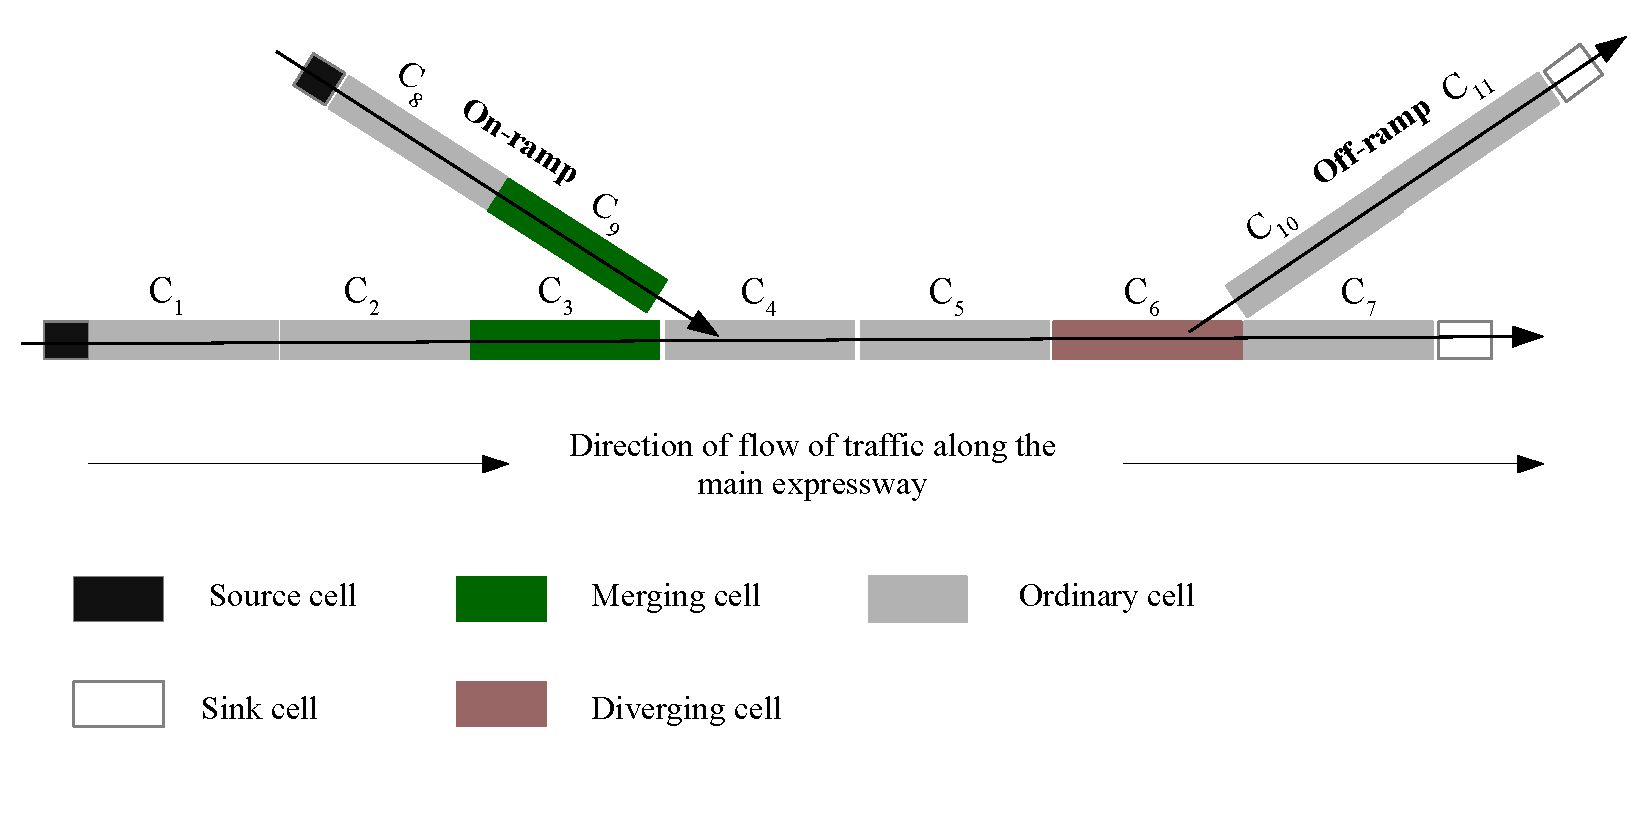
\includegraphics[scale=0.5]{images/cellNetwork.pdf}
	
	\caption{An illustrative cell network.}
	\label{fig:cell-network}
\end{figure*}

In this section we describe our macroscopic traffic flow simulation. Description of the traffic simulator will set up the description of traffic state, action and the reward for the RL agent described in the next section.

The traffic simulator in this work is a faster than wall-clock time macroscopic simulation which is based on the stochastic variant of the Cell transmission model~\cite{boel2006compositional} and METANET~\cite{kotsialos2002traffic}. The cell network $\mathbb{C}$ is comprised of $n$ cells. At each time-step, $k=0,1, .... K$ (where $K$ is the time horizon) the state of all cells are updated. The discrete event simulation time-step used for this simulator is a constant, $k=4$ seconds in all the experiments.

The state of a cell $c_i\in \mathbb{C}$ at each time-step $k$ is determined by the concept of {\it sending} $S_i(k)$ and {\it receiving potentials} $R_i(k)$. $S_i(k)$ and $R_i(k)$ represent the number of vehicles cell $c_i$ can send and receive at time-step $k$. The mean and standard deviation of speed for a cell $c_i$ are denoted by $v_i(k)$ and $v_i^{\text{sd}}(k)$ respectively.  The number of vehicles in a cell $c_i$ at time-step $k$ is given by $N_{i}(k)$. While $N_i^{\text{max}}(k)$ represents the maximum number of vehicles that can be accommodated in cell $c_i$ given an average speed of $v_i(k)$. $N_i^{\text{max}}(k)$ is given by
\begin{equation}
\label{eq:nmax}
N_i^{\text{max}}(k)=\frac{l_i\cdot \lambda_i}{T_{\text{gap}}\cdot v_{i}(k)+ L_{\text{eff}}}
\end{equation}
where $L_{\text{eff}}$ is the {\it effective} vehicle length while $T_{\text{gap}}$ represents the safe time gap.
The length of cell $c_i$ is denoted by $l_i$ which is a variable and subject to the constraint $l_i \ge V_0^i\cdot T$. Where $V_0^i$ is the constant free-flow speed for the cell. This constraint ensures that no vehicle can enter and exit a cell within one time-step. The number of lanes in cell $c_i$ corresponding to the associated road-link is denoted by $\lambda_i$.  Finally $y_i(k)$ represents the number of vehicles that exit a cell $c_i$ during the time interval $k$ through $k+1$, given the average speed in the cell during this time interval is $v_i(k)$.

The cells constituting the cell network $\mathbb{C}$ are classified into five different types as shown in Figure~\ref{fig:cell-network}. Note that this is an illustrative network and not the real-world expressway (see Section~\ref{subsec:pie}) simulated for the experiments. The {\it Merging} cells are associated with the parameter {\it merge priority} $\mu\in [0.0,1.0]$ which controls the proportion of vehicles that moves to the next cell in a given time-step. The {\it Source} and {\it Sink} cells are not physically related to any of the road links but are effectively {\it ghost cells}. The former injects vehicles into the simulation while the vehicles exit the simulation through the latter. Note that the inter-arrival rates of vehicles at all source cells are kept constant during simulation time horizon of $K$ time-steps. A {\it Diverging} cell is associated with the turn ratios $\tau \in [0.0,1.0]$, representing the proportion of vehicles exiting the expressway through off-ramps and those continuing to traverse along the expressway. Cells $C_3$ and $C_9$ are considered {\it predecessors} of cell $C_4$ while cells $C_{10}$ and $C_7$ are considered {\it successors} of cell $C_6$.

Refer to the technical report~\cite{sunderrajan2016symbiotic} for details on the algorithm and equations governing the model of this stochastic traffic simulation. Stochastic noise is added to the function decreasing the mean-flow speed of each cell which results in the creation of spontaneous {\it phantom jams} and shock waves as occurring in real life.





\section{Deep Q-learning for ramp metering}
\label{sec:deep-ql}

In this paper we use the variant of Q-learning called {\it Deep Q-learning} introduced in~\cite{mnih2015human}. Q-learning~\cite{sutton1998reinforcement} is an RL algorithm which is known to converge to the optimal policy. Q-learning is characterized by a set of states $\mathbf{S}$ and actions $\mathbf{A}$.  Q-learning is a {\it model free} technique which learns the action-value (also known as $Q$) function represented by $Q^*(s,a)$ providing the expected utility of taking an action $a\in \mathbf{A}$ in given state $s \in \mathbf{S}$ of the environment and then following the optimal policy there afterwards. 

The basic implementation of Q-learning uses Q-tables to store the action-values. Each row represents the state $s \in \mathbf{S}$ while each column represents the actions $a \in \mathbf{A}$. This approach is not feasible for many real-world control scenarios consisting of hundreds of millions of states. Consider the case of traffic where the state space is continuous and hence infinite. This problem is usually overcome by the use of {\it function approximators} for the action value function represented as $Q(s,a;\theta) \approx Q(s,a)$. The most common function approximators are linear in nature. For stochastic non-linear systems such as traffic, a non-linear function approximator such as neural network can be used. In the case of neural networks $\theta$ represents the weights of the underlying neurons.

For this work, we are inspired by the recent successes of Mnih et.al~\cite{mnih2015human} in effectively training convolutional neural networks (for non-linear function approximation) to achieve human level performance in playing several video games. The \ac{ANN} used in our work for generalizing the state space, enables the ramp metering controller to take the appropriate control action at the on-ramps in expressway sections. The controller for operating the ramp meters is referred to as the DRL-agent henceforth. As pointed out in~\cite{mnih2015human} the \ac{DRL} algorithm uses a biologically inspired technique called {\it experience replay} for {\it off-policy} learning where the agent takes an action $a=max_{a}Q(s,a;\theta)$ with probability $1-\epsilon$ and a random action with probability $\epsilon$ ensuring adequate exploration of the state space.  


In this section we describe the Markov decision process (MDP) for reducing traffic delay using ramp metering. The goal of the DRL-agent is to  minimize the net discounted delay experienced by all vehicles in all cells over a fixed time horizon of $K$ time-steps. The DRL-agent achieves this by learning a policy to determine the appropriate traffic light configuration for all controllable on-ramps depending upon the state in the simulator. The simulator also provides rewards (discussed subsequently) which is used by the DRL-agent to determine the utility of an action taken.

\subsection{Traffic State}
The state of the simulator at time-step $k$ is defined in terms of state of each cell $c_i\in \mathbb{C}$ (except source and sink cells) given by $\frac{n_i(k)}{N_i^{\text{max}}(k)}$. This represents the ratio of the number of
vehicles in $c_i$ to the maximum number of vehicles that can be accommodated in $c_i$ at time-step $k$.
\subsection{Reward Computation}
The total delay $D_{\text{total}}$ over $K$ time-steps is given by
\begin{align}
D_{\text{total}}=\sum\limits_{\substack{k=0}}^{K}\sum\limits_{\substack{i=0}}^{|\mathbb{C}|}d_i(k)
\end{align}
where $d_i(k)$ is the delay experienced by cell $c_{i} \in \mathbb{C}$ at time-step $k$. The delay $d_i(k)$ is given by
\begin{align}
\label{eqn:delay}
d_i(k)=min\Big(0,y_i^{\text{free}}(k)-y_i(k)\Big)
\end{align}

%\todo[inline]{the sums are not entirely correct, because $c_i$ is not used in the last part. it should be something like $\sum_{i = 0}^{|\mathbb{C}|}$
%\\Abhinav's response\\
%Does it look alright now?
%}
The parameter $y_i^{\text{free}}(k)$ represents the number of vehicles that would have exited cell $c_i$ during time-step $k$ if $v_i(k)=V^0_i$. Equation~\ref{eqn:delay} thus represents the number of vehicles affected due to congestion in the cell network in all cells $c_i\in \mathbb{C}$ at time-step


 $k$.


The reward $r_{k+1}$ at the end of time-step $k$ is given by
\begin{equation}
r_{k+1}=\begin{cases}
\frac{(D^{\text{noRM}}_{\text{total}}-D^{\text{RM}}_{\text{total}})}{D^{\text{noRM}}_{\text{total}}}, & \text{if } k=K \\
0, & \text{otherwise}
\end{cases}
\end{equation}
$D_{\text{total}}^{\text{noRM}}$ represents the total delay when no ramp metering is employed while $D_{\text{total}}^{\text{RM}}$ represents the total delay experienced over $K$ time-steps when ramp metering is employed using the policy determined by the \ac{ANN}. The DRL-agent thus tries to learn a ramp metering policy which tries to minimize the total delay experienced by all vehicles over a time horizon of $K$ time-steps in comparison to baseline policy of no ramp metering control. The reward at the end of terminal time-step $K$  is clipped to be in range $-1.0\le r_{K+1}\le 1.0$ as suggested in~\cite{mnih2015human}.



\subsection{Actions and Setup for Reinforcement Learning}

\begin{figure}[!htbp]
	\centering
	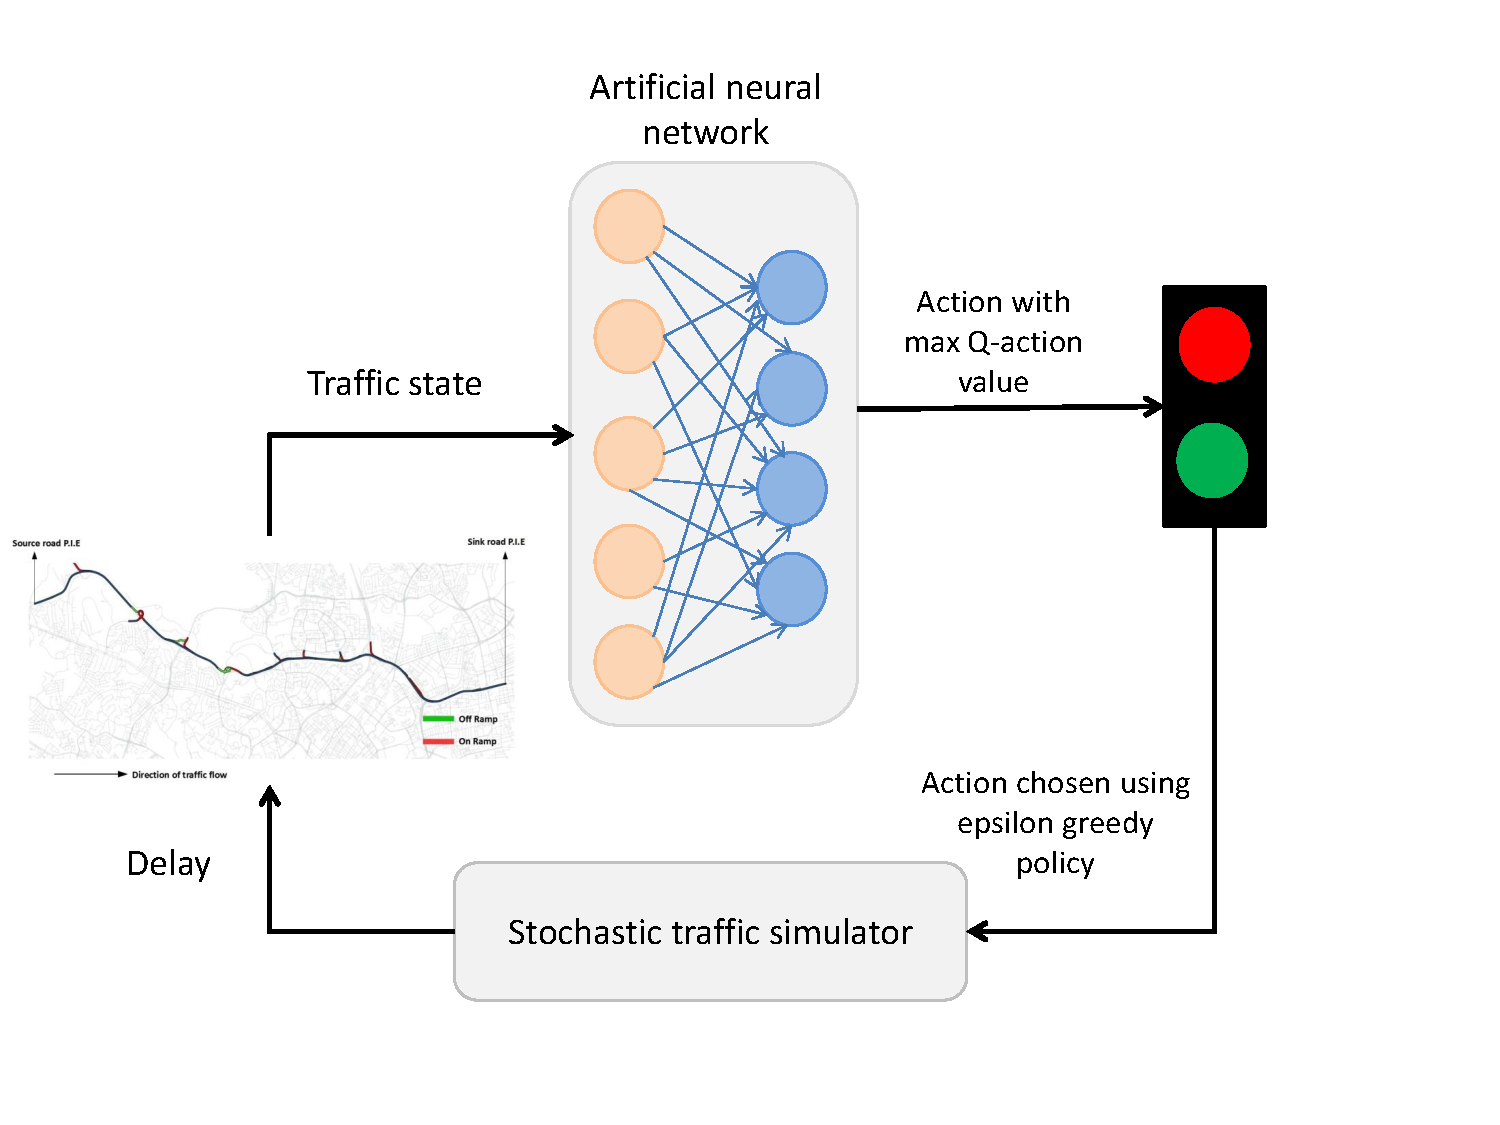
\includegraphics[scale=0.385]{images/DQN-RM.pdf}
	
	\caption{Deep Q-learning for ramp metering.}
	\label{fig:dqn-rm}
\end{figure}

Figure~\ref{fig:dqn-rm} shows the setup for adaptive ramp metering control using deep Q-learning. In our experiments the minimum phase time for each ramp meter is $12$ seconds, i.e. $3$ simulation time-steps. Given that the light at each controllable on-ramp  can either be red or green, the number of actions that can be taken at time-step $k$ is $2^\Psi$ where $\Psi$ denotes the number of controllable on-ramps.
\begin{algorithm}[!t]
	\caption{Deep Q-learning for adaptive ramp metering control.}
	\label{algo:ramp-metering}
	\begin{algorithmic}[1]
		
		\State Initialize replay memory $\mathbb{M}$ of size $32$.
		\State Initialize the neural network (action-value function) $Q$ with weights $\Theta$.
		\State Initialize the target action-value function (another neural network) $\bar{Q}$  for generating $t_j$ with weights $\bar{\Theta}\leftarrow \Theta$.
		
		\Repeat
		\State Set random flow rates at all source cells.
		\State  Warm up traffic simulator.
		\For{$k=0, K$}
		\State Get the state $s_k$ from the cell network in simulator.
		\If{$\text{random}_{\text{double}}<\epsilon$}
		\State Select random action $a_t$ 
		\Else
		\State Select action $a_k=\text{argmax}_{a}Q(s_k,a;\theta)$
		\EndIf
		\State \begin{varwidth}[t]{\linewidth}
			Observe the reward $r_{k+1}$ for the action $a_k$
			
			\hskip\algorithmicindent and the new cell state $s_{k+1}$
		\end{varwidth}
		\State Create transition tuple $\mathbf{T}=(s_k, a_k,r_{k+1}, s_{k+1})$ 
		
		\If{$size(\mathbb{M})<N$}
		\State Add $\mathbf{T}$ to memory $\mathbb{M}$
		\Else
		\State replace first element in $\mathbb{M}$ with the tuple $\mathbf{T}$
		\State Sample random mini-batch $\mathbb{B}$ from $\mathbb{M}$
		\For{\textbf{each} $ \mathbf{T}\in \mathbb{B}$}
		\If {$(j+1)<K$}
		\State $t_j=r_j+\gamma\cdot \text{max}_{a}(\bar{Q}(s_{j+1},a_{j+1};\bar{\Theta}))$
		\Else
		\State $t_j=r_j$
		\EndIf
		\State \begin{varwidth}[t]{\linewidth}
			Use $(t_j-Q(s_j,a_j;\Theta))^2$ for gradient 
			
			\hskip\algorithmicindent descent with respect to $\Theta$.
		\end{varwidth}
	\EndFor
		\State After $C$ steps, reset $\bar{Q}\leftarrow Q$ 
		
		\EndIf
		
		
		\EndFor 
		\Until{$\text{epoch}<\text{epoch}_{\text{max}}$}
		
	\end{algorithmic}
\end{algorithm}

After $3$ simulation time-steps the traffic simulator gives the state of each of cell $c_i \in \mathbb{C}$ (excluding source and sink cells) as an input to the \ac{ANN}.  As mentioned previously, traffic state at time-step $k$ is given by the ratio of number of vehicles to the maximum number of vehicles that an be accommodated in a cell (for the current traffic speed) for all cells belonging to the cell network $\mathbb{C}$. The state space is infinite since the ratios $\frac{n_i(k)}{N_i^{\text{max}}(k)}$ (representing the state) for all cells are real valued and continuous. The output layer of the \ac{ANN} consist of $2^\Psi$ neurons representing the number of actions that the DRL-agent can make. The action $a$ is chosen from \ac{ANN} output based on the $\epsilon$ greedy (see lines $9$ through $12$ of~Algorithm~\ref{algo:ramp-metering}) policy. The traffic light combination corresponding to the output of the \ac{ANN} is given as an input to the traffic simulator which computes the next state and the delay incurred in subsequent $3$ time-steps. 

Considering that the DRL-agent acquires the traffic state of all cells of the expressway and controls the $\Psi$ controllable on-ramps simultaneously, the DRL-based ramp metering is a multivariable regulator ramp metering strategy.

Refer to Algorithm~\ref{algo:ramp-metering} implementing experience replay for training the DRL-agent for ramp metering control. To perform experience replay,  we store the DRL-agent's experience as a transition tuple  $\mathbf{T}=(s_t, a_t,r_{t+1}, s_{t+1})$ to the replay memory data store $\mathbb{M}$.  The standard RL assumption that future rewards are discounted by a constant factor $\gamma=0.99$ is made. See~\cite{sutton1998reinforcement} for more details regarding discounting future rewards during Q-learning. During the training process, random mini batches $\mathbb{B}$ of size $32$  are sampled  from  $\mathbb{M}$. Experience replay thus avoids the pitfall of learning from consecutive samples which are strongly correlated. As suggested in~\cite{mnih2015human}, two artificial neural networks are used to improve the stability of the learning process. The \ac{ANN} $Q$ with weights $\Theta$ represents the action-value function $Q$ while the \ac{ANN} $\bar{Q}$ with weights $\bar{\Theta}$ generates the Q-learning targets $t_j$ (see line $22$ of Algorithm-~\ref{algo:ramp-metering}). The weights of the \ac{ANN} $\bar{Q}$ are replaced with those of $Q$ every $C=50$ steps. Note that $\text{epoch}$ refers to one forward pass and one backward pass of the neural network over the mini batch $\mathbb{M}$.

\begin{table*}[!htbp]
	\centering
	\caption{Hyper-parameters used for deep Q-learning.}
	\label{table:hyper-param}
	\begin{tabular}{@{}lll@{}}
		\toprule
		\multicolumn{1}{c}{\textbf{Hyper Parameter}} & \multicolumn{1}{c}{\textbf{Value}} & \multicolumn{1}{c}{\textbf{Description}}                                                                                                                                                                                              \\ \midrule
		Number of hidden layers                      & 2                                  & \begin{tabular}[c]{@{}l@{}}The number of hidden layers in the neural network used for \\ Deep Q-learning. The first hidden layer consists of $200$ neurons\\ while the second hidden layer is composed of $150$ neurons.\end{tabular} \\
		Learning rate                                & 0.00025                            & Learning rate used by the RMSProp algorithm.                                                                                                                                                                                          \\
		Discount factor                              & 0.98                               & Discount factor used in Q-learning update.                                                                                                                                                                                            \\
		Replay memory size                           & 1500000                             & \begin{tabular}[c]{@{}l@{}}Stochastic gradient descent updates are sampled from this number \\ of recent $(s_t, a_t,r_{t+}, s_{t+1})$  tuples stored in memory.\end{tabular}                                                                      \\
		Mini batch size                              & 32                                 & \begin{tabular}[c]{@{}l@{}}The batch size used by the  stochastic Gradient descent (SGD) \\ update of neural network weights.\end{tabular}                                                                                            \\
		RMS decay                                    & 0.95                               & Gradient momentum used by the RMSProp algorithm.                                                                                                                                                                                      \\
		Initial exploration                          & 1.0                                & The initial $\epsilon$ in the $\epsilon$ greedy evaluation.                                                                                                                                                                           \\
		Final exploration                            & 0.05                                & The final $\epsilon$ in the $\epsilon$ greedy evaluation.                                                                                                                                                                              \\
		Target network update frequency              & 100                                 & \begin{tabular}[c]{@{}l@{}}The frequency with which target network (in number of steps) is\\ evaluated.\end{tabular}                                                                                                                  \\ \bottomrule
	\end{tabular}
	%\todo[inline]{Shouldn't the first word of the first column also be capitalized?}
\end{table*}




\section{Experiments}
\label{sec:experiments}

In this section we begin with a description of the hyper-parameters used for training the DRL-agent. Description of the experimental setup, the training process of the DRL-agent, evaluation of the DRL-agent's performance followed by a brief discussion of the results of evaluation. The details of the hyper-parameters used for training the DRL-agent (as described in Algorithm~\ref{algo:ramp-metering}) are shown in Table~\ref{table:hyper-param}. The \ac{ANN} consists of two hidden layers with sizes equal to $200$ and $150$ neurons each. The size of the input layer is equal to the number of physical cells in the simulated expressway section. The size of  the output layer corresponds to the number of actions that the DRL-agent can take at each state. The size of the output layer is thus $2^\Psi$ as explained previously. The hidden layers of the \ac{ANN} employ {\it leaky rectified linear unit} (ReLU) as the activation function for each neuron. The output layer uses the {\it identity} activation function which is commonly used for regression problems.





\subsection{The Simulated Environment}
\label{subsec:pie}
\begin{center}
	\begin{figure}[!htbp]
		\centering
		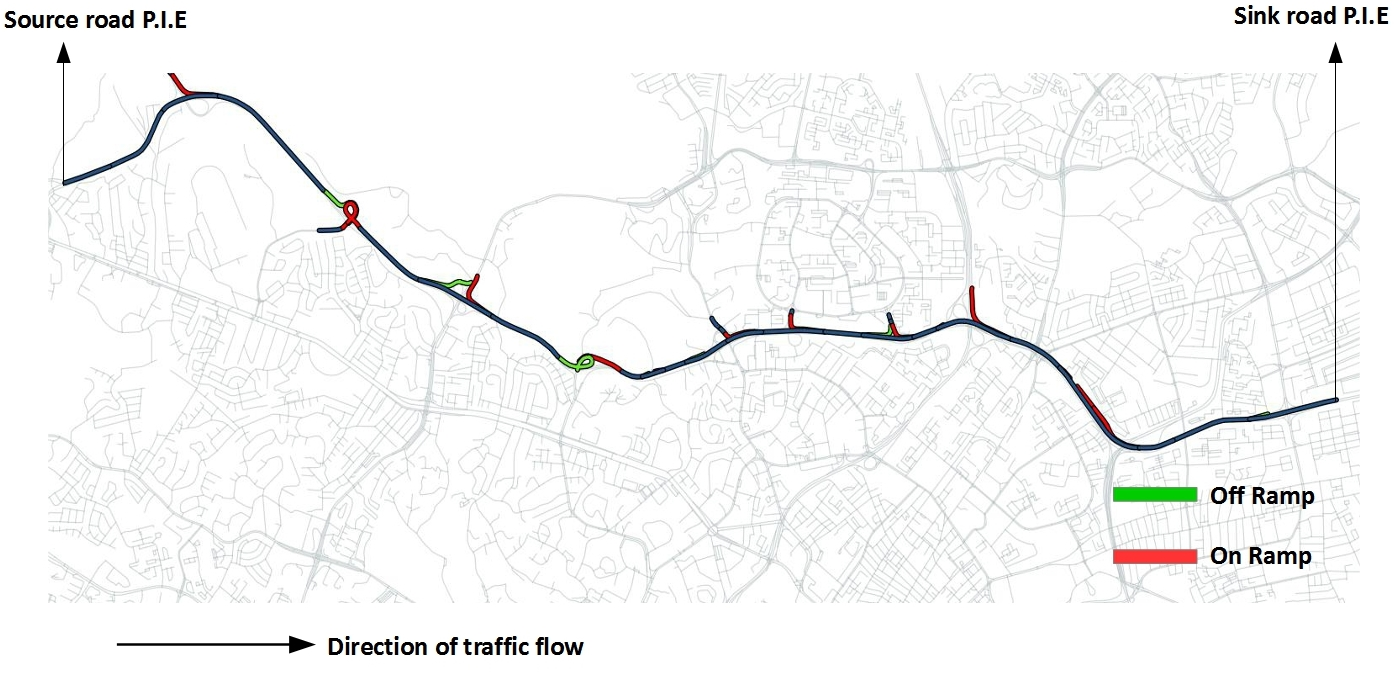
\includegraphics[scale=0.28]{images/PIE.jpg}
		\captionsetup{justification=centering}
		\caption{Simulated $13$ km section of P.I.E. (Singapore) and location of all on/off-ramps.}
		\label{fig:pie-changi}
	\end{figure}
\end{center}

For the experiments in this report, we simulate a $13$ km stretch of P.I.E. (Pan Island Expressway) in central Singapore (Figure~\ref{fig:pie-changi}) with all on and off-ramps. The on-ramps and the first P.I.E. link are sources, while all off-ramps and the last link on P.I.E. are sinks. Refer to the Table~\ref{table:iat} for the location of all on/off-ramps starting from the beginning of the first road-segment on P.I.E. The average distance between two on-ramps is around $565\text{~m}$ along this stretch of P.I.E. The turn ratios for all off-ramps is kept constant at $\tau=0.25$. This implies that $25\%$ of all vehicles exit at a given off-ramp while the remaining $75\%$ of the vehicles continue to travel on the main expressway. The number of lanes in the simulated stretch of the expressway varies between $3$ and $6$. The total number of cells  in the cell network for the expressway section simulated (including on/off-ramps and excluding the source and link cells) is $212$.

\subsection{Traffic Scenario}

\begin{table}[!htbp]
	\centering
	\caption{Mean flow rates at all on-ramps.}
	\label{table:iat}
	\begin{tabular}{@{}lll@{}}
		\toprule
		\multicolumn{1}{c}{\textbf{Distance (m)}} & \multicolumn{1}{c}{\textbf{Ramp type}}                          & \multicolumn{1}{c}{\textbf{\begin{tabular}[c]{@{}c@{}}Flow\\ (vehicles/hour)\end{tabular}}} \\ \midrule
		0.0                                       & First P.I.E. link                                                & 3600 - 4000                                                                                 \\
		583.98                                    & On-ramp                                                         & 1100-1600                                                                                   \\
		2489.87                                   & On-ramp                                                         & 1100-1600                                                                                   \\
		4071.9                                    & \begin{tabular}[c]{@{}l@{}}Controllable \\ on-ramp\end{tabular} & 800 - 1100                                                                                  \\
		5531.18                                   & On-ramp                                                         & 1100-1600                                                                                   \\
		5965.29                                   & On-ramp                                                         & 1100-1600                                                                                   \\
		7025.15                                   & On-ramp                                                         & 1100-1600                                                                                   \\
		7658.4                                    & \begin{tabular}[c]{@{}l@{}}Controllable\\ on-ramp\end{tabular}  & 800 - 1100                                                                                  \\
		8554.28                                   & \begin{tabular}[c]{@{}l@{}}Controllable\\ on-ramp\end{tabular}  & 800 - 1100                                                                                  \\
		9591.84                                   & On-ramp                                                         & 1100-1600                                                                                   \\
		11286.2                                   & On-ramp                                                         & 1100-1600                                                                                   \\
		11286.2                                   & \begin{tabular}[c]{@{}l@{}}Controllable\\ on-ramp\end{tabular}  & 800 - 1100                                                                                  \\ \bottomrule
	\end{tabular}
	%\todo[inline]{On ramp -> On-ramp}
\end{table}
Table~\ref{table:iat} lists the range of mean in-flow rates in vehicles/hour for all source links. The mean flow rates for an episode of the simulation is picked randomly within the specified range and kept constant during the simulated time horizon for all experiments (training as well as evaluation) in this paper. Notice that the flow of vehicles into the expressway along all $\Psi=4$ controllable on-ramps is less than that of the ones which do not have ramp meters.

\begin{figure}[!htbp]
	\centering
	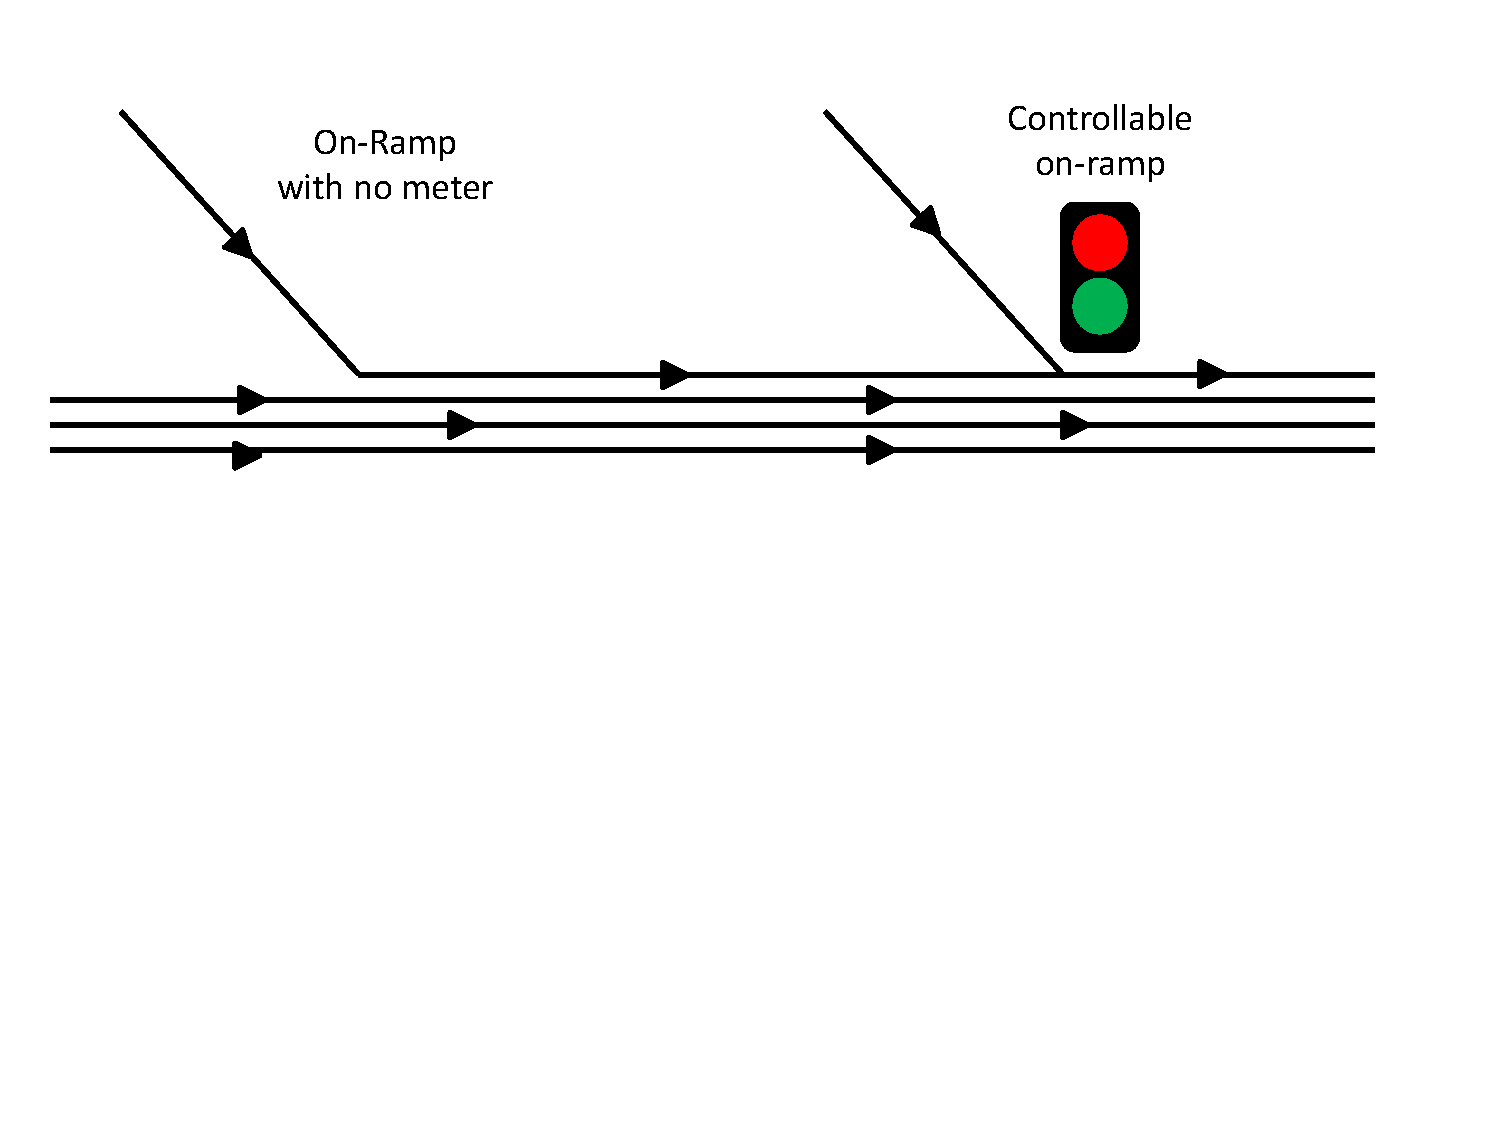
\includegraphics[clip=true,trim=0.3cm 11cm 1cm 0.0cm,scale=0.35]{images/Ramps.pdf}
	
	\caption{Structure of on-ramps in the traffic simulation.}
	\label{fig:ramp-struc}
\end{figure}

Figure~\ref{fig:ramp-struc} illustrates the difference between a controllable on-ramp and an ordinary one with no traffic light. Vehicles entering the P.I.E along an on-ramp with no ramp meter cause lesser disruption to the main line flow compared to the on-ramps with meters due to the presence of an extra lane.




\subsection{Training}
\label{subsec:training}

%\todo[inline]{There needs to be a sentence here. Something like: ''In order for the ANN to determine the actions during run-time, the network has to be trained first.'' Which data did we train the ANN on? Was the training data generated the same way as our validation data? How do we avoid over-fitting?}



\begin{figure}[b]
	\centering
	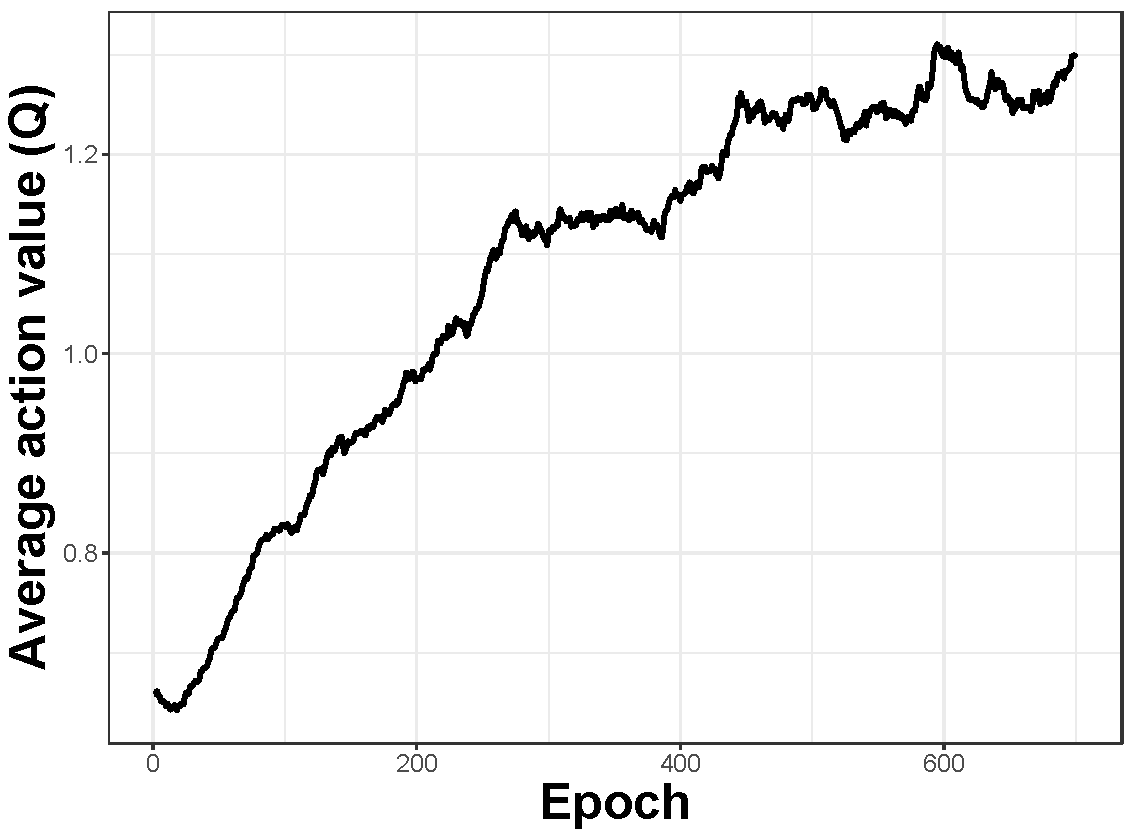
\includegraphics[scale=0.35]{images/Qvalue.pdf}
	
	\caption{Average action-value.}
	\label{fig:q-value}
\end{figure}
The \ac{ANN} is trained to determine the appropriate action when the traffic state from all the cell network (except the source and sink) are given to it as inputs. The output of the \ac{ANN} is used to determine the actions based on the $\epsilon$ greedy strategy. Figure~\ref{fig:q-value} plots the action-value function $Q$ which provides an estimate of how much discounted reward a DRL-agent can get by taking an action $a$ in a state $s$ and following the policy from there onwards. As suggested in~\cite{mnih2015human} we collect a fixed set of states  before training starts to track the average of the maximum predicted action-value for these states.
A smooth increase in the $Q$-value which stabilizes after epoch $450$ suggests that deep Q-learning is able to train our \ac{ANN} using stochastic gradient descent in a stable manner despite the lack of any theoretical convergence guarantees.
%\todo[inline]{Is this really proof or just indication?}
For Figure~\ref{fig:q-value}, the average flow rates for all sources were randomly sampled in the ranges specified in Table~\ref{table:iat}. As previously stated, the mean inter-arrival times (and thus flow rates) for all source links/cells are kept constant for an episode of $K$ time-steps.

%\pagebreak

\subsection{Evaluation}
\label{subsec:results}

As explained in Section~\ref{sec:deep-ql}, the goal of our reinforcement learning algorithm is to determine a ramp-meter policy which tries to reduce the total delay $D_{total}$ (in comparison to the no control case) experienced by all vehicles over a time horizon of $k=K$ time-steps. At the end of the training over 500 epochs, we sampled random flow rates (for the source cells) within the ranges specified in Table~\ref{table:iat} and conducted $800$ trials to compare the delays experienced by the vehicles with and without ramp metering. The ramp metering policy is determined by the trained \ac{ANN} which uses the traffic state as input to determine the appropriate traffic lights for the $4$ controllable on-ramps. The \ac{ANN} chooses the action corresponding to the maximum Q-Value for each state with a probability of $0.999$ and chooses a random action otherwise. This is done in order to avoid over fitting.


\begin{figure*}[!htbp]
	
	\subfloat[For all cells including on and off ramps]{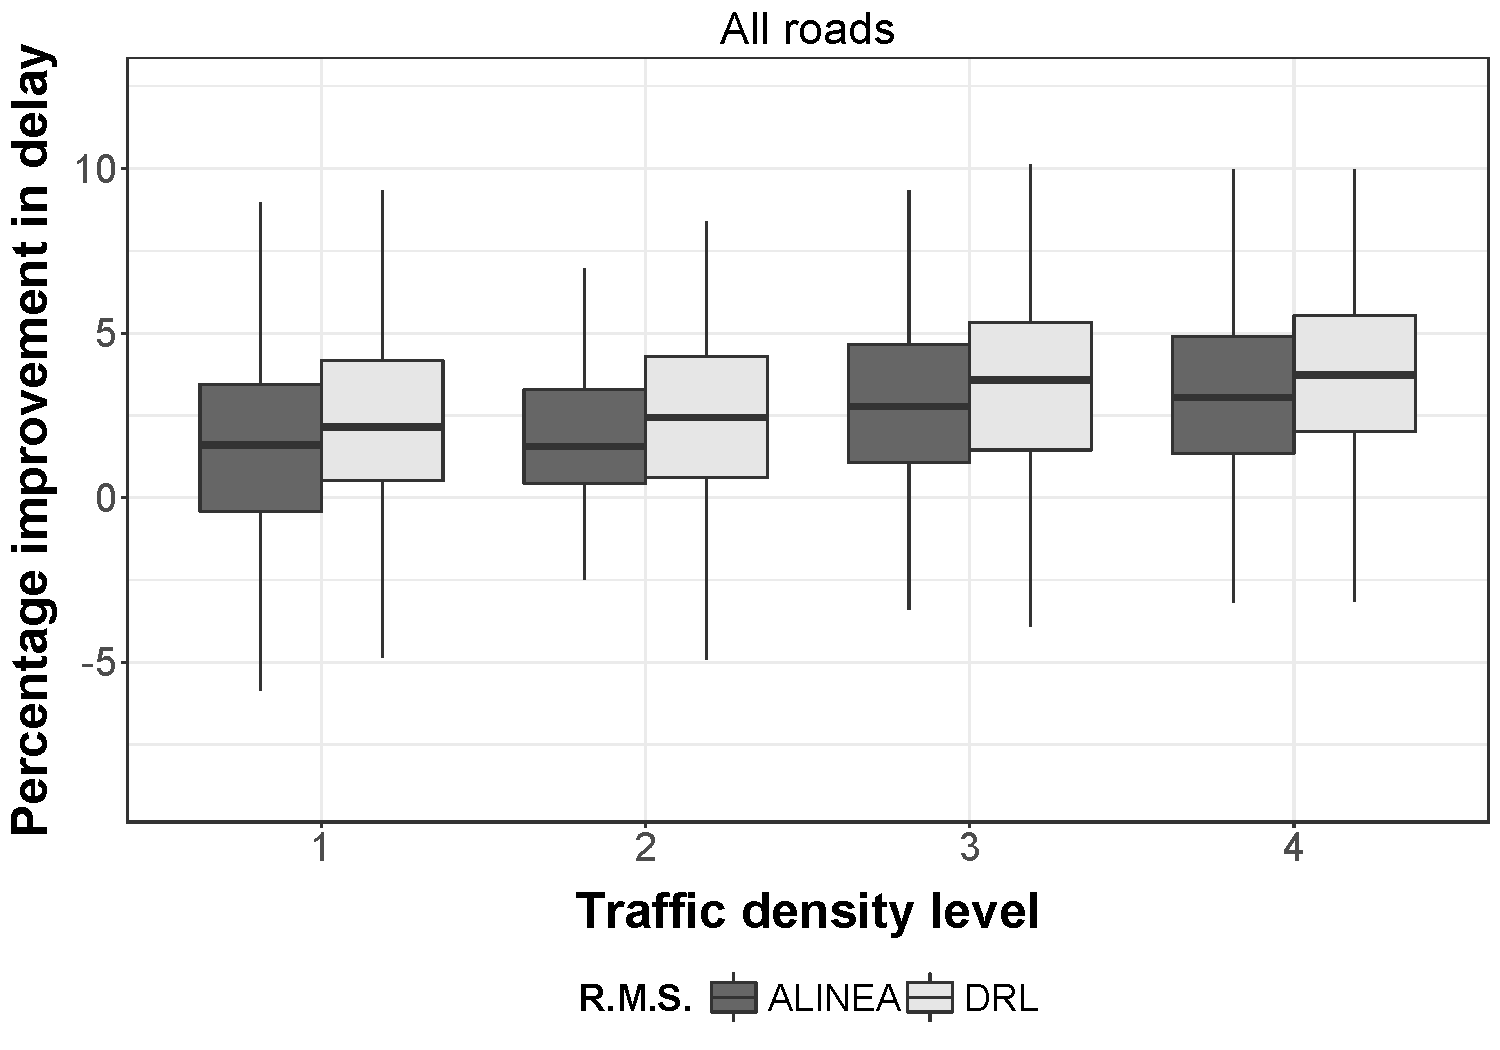
\includegraphics[width=.32\textwidth]{all-roads.pdf}\label{fig:all-roads-delay}}%
	\hfill%
	\subfloat[For the cells constituting expressway section only]{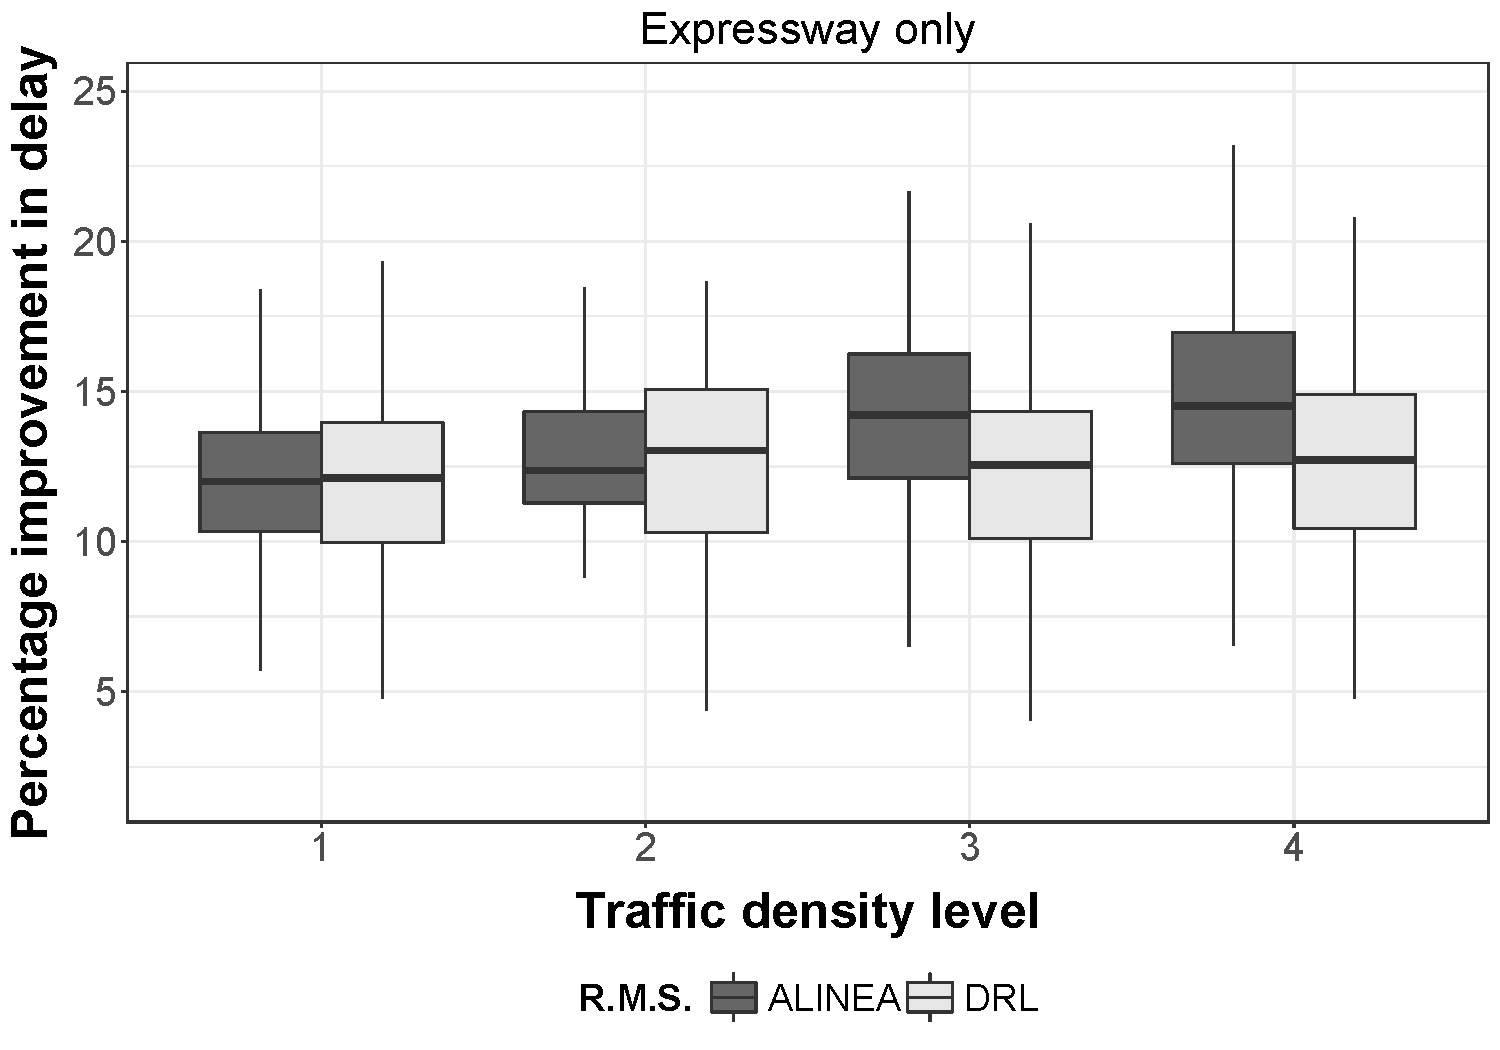
\includegraphics[width=.32\textwidth]{expressway.pdf}\label{fig:only-expressway}}%
	\hfill%
	\subfloat[For the cells constituting the on-ramps only]{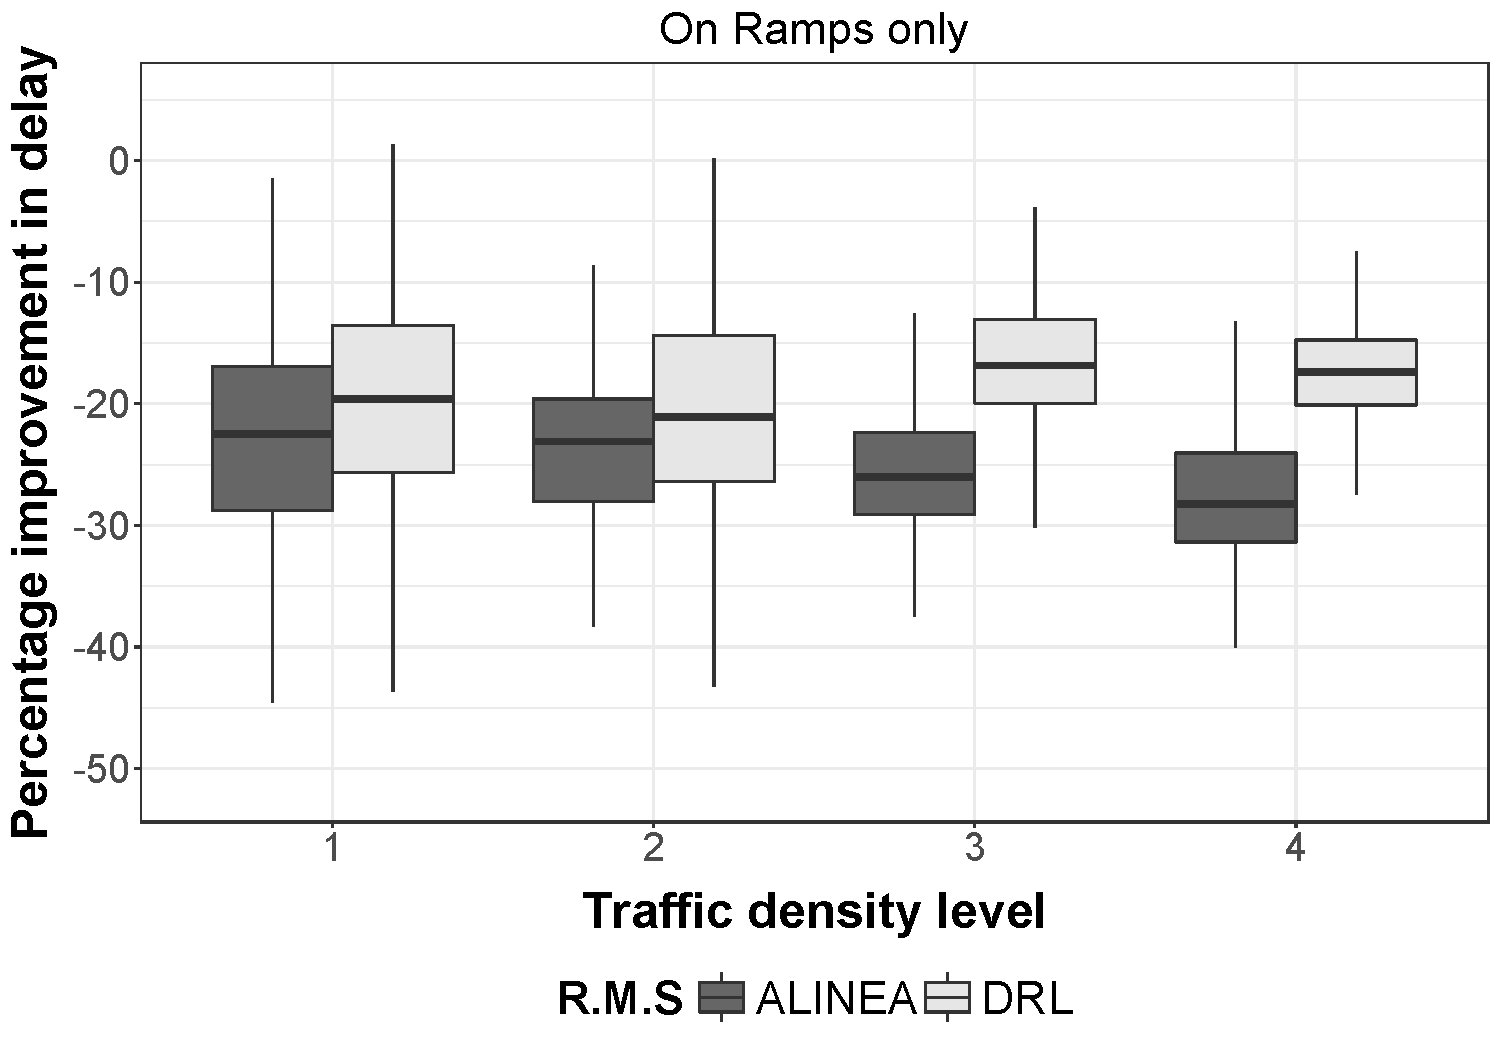
\includegraphics[width=.32\textwidth]{on-ramps.pdf}\label{fig:on-ramps}}%
	\caption{Percentage of delay reduction for the two ramp metering strategies (RMS) DRL and ALINEA.}
	\label{fig:delays}
\end{figure*} 


% Please add the following required packages to your document preamble:
% \usepackage{booktabs}
\begin{table}[!hb]
	\centering
	\caption{Mean traffic density level.}
	\label{table:density-level}
	\begin{tabular}{@{}ccc@{}}
		\toprule
		\textbf{\begin{tabular}[c]{@{}c@{}}Traffic density \\ level\end{tabular}} & \textbf{\begin{tabular}[c]{@{}c@{}}Density range\\ (veh/km/lane)\end{tabular}} & \textbf{Traffic State} \\ \midrule
		1                                                                         & {[}30, 34{]}                                                                    & Synchronized flow      \\
		2                                                                         & (34-38{]}                                                                      & Synchronized flow      \\
		3                                                                         & (38-42{]}                                                                      & Synchronized flow      \\
		4                                                                         & (42-46{]}                                                                      & Congested              \\ \bottomrule
	\end{tabular}
\end{table}

As stated earlier, we implemented the local ramp metering strategy of ALINEA(Equation~\ref{eq:alinea}). We chose the constant regulator parameter $K_R=70.0$ based on~\cite{papageorgiou1997alinea}. Figure~\ref{fig:all-roads-delay} compares the percentage improvement in the overall delay (for all roads including the on/off ramps) for the ramp metering policy determined by the DRL-agent and that of ALINEA over the no ramp metering case for different mean traffic-density levels ranging from synchronized flow to congested (see Table~\ref{table:density-level}). The number of trials in each traffic density level numbers $200$ for ALINEA and DRL. Note that the simulation seeds were changed for each of the $800$ trials ($200$ in each traffic density category) to take into account the stochasticity associated with the traffic flow simulator. The overall median improvement for the DRL-based ramp metering strategy is comparatively better than ALINEA.

Figure~\ref{fig:delays} shows the results of our simulation study in terms of relative delay experienced by the vehicles compared to an approach where no ramp metering is applied.
We observe that the overall delay reduction (Figure~\ref{fig:all-roads-delay}) is similar for ALINEA and \ac{DRL}, with indications of \ac{DRL} performing slightly better.
Figure~\ref{fig:only-expressway} compares the delay experienced over the mainline expressway cells only between ALINEA and \ac{DRL}.
The results indicate that the median delay experienced over the expressway is lower for ALINEA especially at higher traffic density levels of $3$ and $4$.
The reason for the delay benefit over the expressway becomes apparent in Figure~\ref{fig:on-ramps} where  the median delay for the on-ramps is higher for ALINEA (compared to \ac{DRL}) for the traffic density level $3$ and $4$.
In summary, ALINEA trades a higher delay on the on-ramps to achieve better performance on the expressways.
However, this leads to an overall delay for all vehicles that is higher than what we observe using our \ac{DRL} approach, where the delay of each car is treated equally.
We can tune the algorithm to favor the reduction of delay of the expressway cells  over those on the on/off-ramps by weighting the expressway cell(s) delay by a factor $f>1.0$. This will come at the cost of increased delay along the on-ramps potentially causing spillovers to the urban street network which we want to avoid.%\todo for David


Figures~\ref{fig:density-delay} plots the variation of delay for all cells as the average traffic density (in veh/km/lane) is gradually increased from  levels $1$ through $4$ and beyond over $1800$ seconds for different ramp metering strategies. Note that the results of Figures~\ref{fig:density-delay} are averaged over $5$ different trials of the simulator with varying simulation seeds to account for the model stochasticity. The simulated scenario represents a typical rush hour  where the traffic state goes from synchronized flow to congested in a short period of time. We observe that the performance of both ALINEA and \ac{DRL} for overall delay are comparable for densities up until $45$ veh/km/lane corresponding to a synchronized traffic flow regime. \ac{DRL} actually performs better than ALINEA when the traffic conditions are congested for densities beyond $45$ veh/km/lane by adaptively varying the traffic lights at all $4$ controllable on-ramps.

\begin{figure}[!t]
	\centering
	\subfloat[Average traffic density in the rush hour scenario]{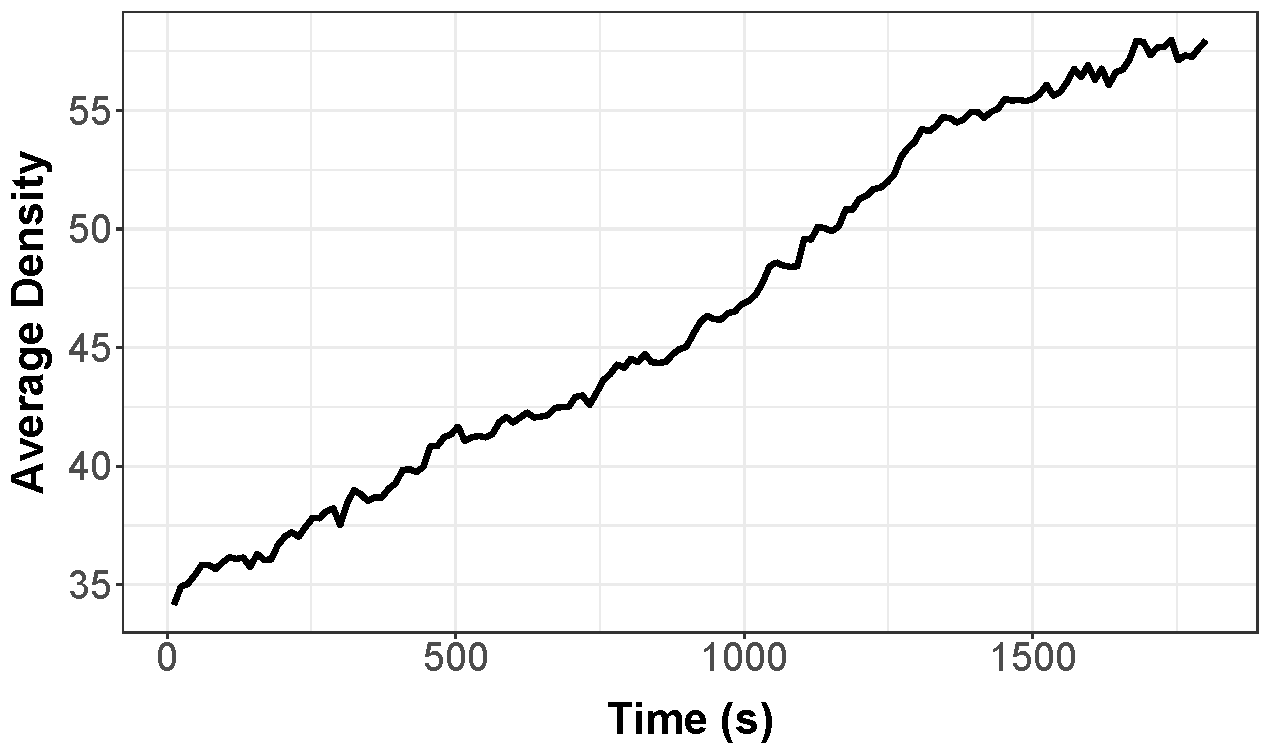
\includegraphics[width=.93\columnwidth]{density-delay2.pdf}}
	\qquad
	\subfloat[Delay experienced by all vehicles in the simulation]{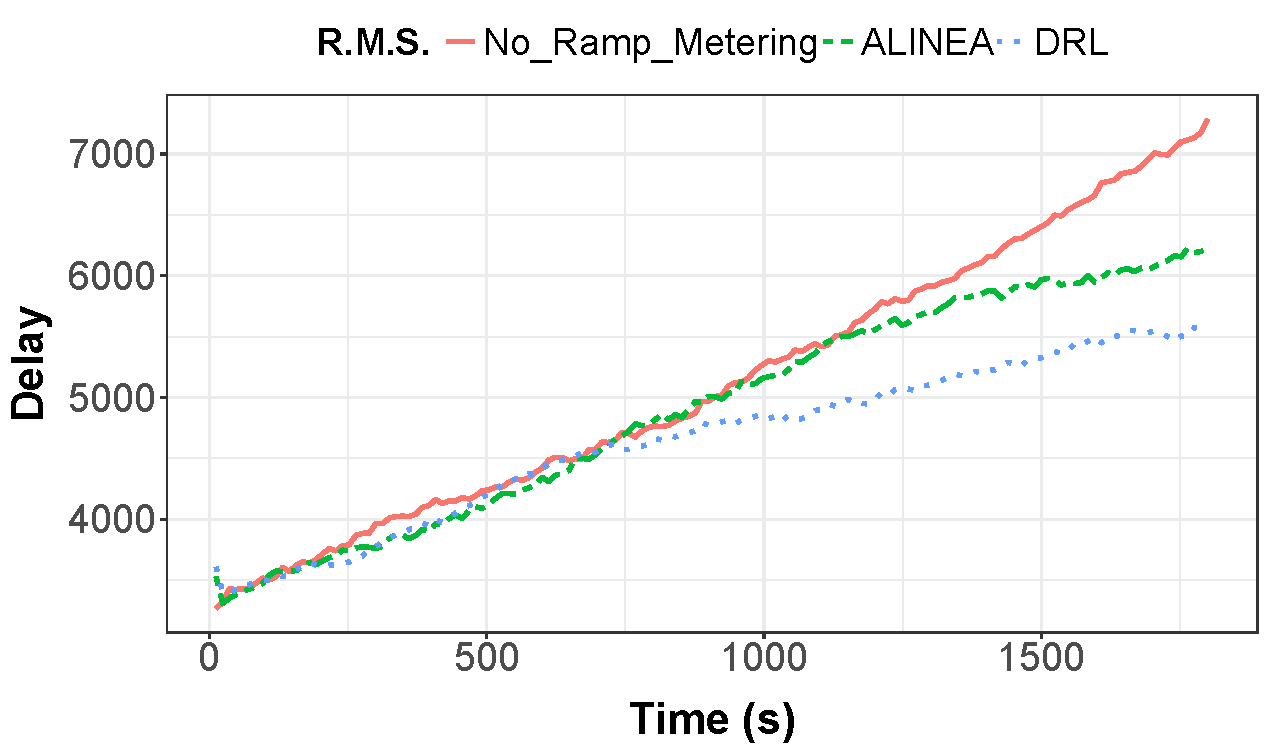
\includegraphics[width=.93\columnwidth]{images/density-delay1.pdf}}
	\caption{Overall delay for different ramp metering strategies as traffic density is gradually increased over $1800$ seconds.}
	\label{fig:density-delay}
\end{figure}



\subsection{Discussion Of Results}
\label{subsec:results-discussion}


The evaluation of the results shows that deep Q-learning is able to learn a policy to minimize the overall and mainline expressway delays over a simulated time horizon of $K$~time-steps. The results also show that deep Q-learning has generalized well given random traffic flows at the sources and the inherent stochasticity in the simulator which causes spontaneous emergence of jams. Encouragingly, the performance of \ac{DRL} is comparable to ALINEA, a widely deployed and successful ramp metering strategy for synchronized traffic flow conditions. Our simulations show that \ac{DRL} performs better than ALINEA when the traffic flow regime is congested.   

The objective of this paper is to show that deep Q-learning can be used to determine model-free policies for ramp metering despite the inherent randomness in traffic systems. There are reasonable chances that the policy determined may not be optimal due to the lack of any theoretical guarantees since \ac{ANN} is employed for function approximation. 




\section{Conclusion and future work}
\label{sec:conclusion}
In this paper, we explored the possibility of applying deep Q-learning for ramp metering and showed that it has the potential for true adaptive real-time traffic control under uncertainty. Deep Q-learning as demonstrated by the recent successes in training computers to pay video games helps us overcome the disadvantages associated with quantizing the near infinite state space. 

%more detailed
We simulated a real-word expressway in the city-state of Singapore using a cell based traffic flow model, which offers fast and efficient performance when used in computer simulations at a macroscopic scale.
This efficiency allowed us to run the high number of iterations required for deep Q-learning to converge.
We found that for different traffic densities, our approach is indeed feasible and produces similar results as the widely used local ramp metering strategy ALINEA. In fact, under dynamic traffic conditions, e.g., at the beginning of the rush hour, our approach outperformed ALINEA yielding a lower delay for all vehicles.

This work has the potential to be extended for other optimal traffic control strategies in urban environments through adaptive traffic signal timings.
Other control strategies that can be investigated for efficacy include variable speed limits, congestion aware routing and traffic signal timing optimization.
Additionally, our approach can be altered using different reward functions, e.g., weighing delays on-ramps or expressways differently.

%\todo[inline]{Add one sentence that we tackle the state space quantization using deep Q-learning because of recent successes in video games}



\appendices
\section*{}
\begin{table}[!h]
	\centering
	\caption{List of important symbols used in the paper.}
	\label{my-label}
	\resizebox{\columnwidth}{!}{%
		\begin{tabular}{p{1.5cm}p{6cm}}
			\toprule
			\textbf{Symbol}                  & \textbf{Explanation}                                                                                                                                                                                                      \\ \midrule
			$k$                              & Constant simulator time-step.                                                                                                                                                                                                                                                                                                                                                                                    \\
			$c_i$                            & A cell belonging to the cell network $\mathbb{C}$.                                                                                                                                                                         \\
			$l_i$                            & Length of  $c_i$.                                                                                                                                                                                                      \\
			$\lambda_i$                      & Number of lanes in  $c_i$.                                                                                                                                                                                             \\
			$v_i(k)$                         & The average speed of vehicles in $c_i$ at  $k$.                                                                                                                                                              \\
			$\rho_i(k)$                         & The vehicle density in $c_i$ at  $k$.                                                                                                                                                              \\
			$n_i(k)$                         & Number of vehicles in $c_i$ at $k$.                                                                                                                                                                         \\
			$N_i^{\text{max}}(k)$            & Maximum number of vehicles that can be accommodated in $c_i$ at $k$.                                                              \\                                                                                                                                                                                         
			$V^0_i$                          & The free-flow velocity of $c_i$.                                                                                                                                                                                    \\
			$y_i(k)$                         & The outflow  from $c_i$ during $k$.                                                           \\
			$y_i^{\text{free}}$              & The outflow from $c_i$ during $k$ given $v_i(k)=V^0_i$.                                                                                                                                                               \\
			$d_i(k)$                         & Delay experienced in $c_i$ during $k$.                                                                                                                                                                                     \\
			$D_{\text{total}}$               & Sum of total delay experienced by all cells over the entire time horizon.                                                                                                                                                  \\
			$S_i(k)$                         & The sending potential of $c_i$ at $k$.                                                                                                                                                                    \\
			$R_i(k)$                         & The receiving potential of $c_i$ at  $k$.                                                                                                                                                                                                                                                                                                                                       \\
			$y^{\text{on}}_{\text{ramp}}(k)$ & Flow from the on-ramp on to the expressway.                                                                                                                                                                                \\
			$K_R$                            & ALINEA constant regulator parameter.                                                                                                                                                                                       \\
			$Q(s,a)$                         & Action value or Q function.                                                                                                                                                                                                \\
			$s$                              & A state $s \in \mathbf{S}$ of the environment.                                                                                                                                                                             \\
			$a$                              & An action $a \in \mathbf{A}$ the DRL-agent  can make.                                                                                        \\
			$Q(s,a;\theta)$                  & A Q function using a nonlinear function approximator such as an \ac{ANN}. Here $\theta$ represents the weights  of an \ac{ANN} used for state space approximation. \\
			$\Psi$                           & Number of controllable on-ramps.         
			\\
			$\gamma$ & The discount factor for future rewards                                                                                                                                                            \\ \bottomrule
	\end{tabular}}
\end{table}




% use section* for acknowledgment
\section*{Acknowledgment}
This work was financially supported by the Singapore National Research Foundation under its Campus for Research Excellence And Technological Enterprise (CREATE) programme.

%\todo[inline]{Some figures have a full stop in their caption in the end, some don't. unitize please (go for full stops for the big captions, and no-full stop for the sub-captions}

%\todo[inline]{In your illustrations (Fig 1, 2, 4) you alter between title case and no-title case. unitize please}


% Can use something like this to put references on a page
% by themselves when using endfloat and the captionsoff option.
\ifCLASSOPTIONcaptionsoff
  \newpage
\fi



% trigger a \newpage just before the given reference
% number - used to balance the columns on the last page
% adjust value as needed - may need to be readjusted if
% the document is modified later
%\IEEEtriggeratref{8}
% The "triggered" command can be changed if desired:
%\IEEEtriggercmd{\enlargethispage{-5in}}

% references section

% can use a bibliography generated by BibTeX as a .bbl file
% BibTeX documentation can be easily obtained at:
% http://mirror.ctan.org/biblio/bibtex/contrib/doc/
% The IEEEtran BibTeX style support page is at:
% http://www.michaelshell.org/tex/ieeetran/bibtex/
%\bibliographystyle{IEEEtran}
% argument is your BibTeX string definitions and bibliography database(s)
%\bibliography{IEEEabrv,../bib/paper}
%
% <OR> manually copy in the resultant .bbl file
% set second argument of \begin to the number of references
% (used to reserve space for the reference number labels box)
%\begin{thebibliography}{1}
\bibliographystyle{IEEEtran}
\bibliography{deeprl} 

%\end{thebibliography}


% that's all folks
\end{document}


